\documentclass[a4paper]{article}

\usepackage[english]{babel}
\usepackage[utf8]{inputenc}
\usepackage{amsmath}
\usepackage{graphicx}
\usepackage{algorithm}
\usepackage{algpseudocode}

\title{Methods for Geometry-Independent Microstructure Control}

\author{William Halsey, James Ferguson, Alex Plotkowski, Vincent Paquit, Ryan Dehoff}

\date{\today}

\begin{document}
\maketitle

\begin{abstract}
The ability to manipulate the formation of microstructure is one of the potential advantages of additive manufacturing. However, the additive manufacturing process is riddled with complex interactions between machine parameters, geometry, and print order to name a few. TODO. This work explores a set of general algorithms that may be used to manipulate the formation of arbitrary microstructures regions. We can accomplish these aims through the manipulation of print order and timing alone. Our approaches do not require unique parameters for each microstructure region. We employ analytical models and combine it with two distinct iterative methods for manipulating the print path the yield the desired microstructure regions. 
\end{abstract}


\section{Introduction}
\label{sec:intro}

Additive manufacturing has allowed for the possibility of tailoring the structural characteristics of a part. Specifically, AM has the potential to enable the formation of different microsturcture in distinct regions of a part. This can have wide-ranging impact within manufacturing.

Additive manufacturing offers the most flexibility of any manufacturing process. It enables the fabrication of geometries that are not possible with conventional methods of manufacturing. Further more, the process allows for the possibility of controlling the formation of microstrucutre for a component during fabrication. In fact, [blank] has also shown the ability ot utilize custom infill pattern for metal additive manufacturing. specifically, they use a spot fill patter that does not rely on the "black box" of software imposed by additive manufacturing machine manufacturers. They deomnstrated how using sucha a technique can allow for the production of either columnar grains with anisotropic tendencies or equiaced grains with isotropic tendencies. However, their approach has limited flexibility because the algorithm of their infill pattern necessitates that the geometry is square or a similarly simple geometry. Additionally, their approach only allows for homogeneous microstrucutre within a layer of a part. [blank] has shown that through metal additive processes that the very microstructure of a part can be controlled and different regions of a layer can have certain mechanical properties imposed upon them. However, the technique employed there is dependant on the proprietary algorithms of ARCAM (wat is arcam? need to introduce some of the concepts better. This paper introduces a method of microstructure control that is more general than any of these previous efforts. It utilizes the spot infil method (as opposed to proprietary rasterization techniques).

\cite{dehoff2015site} has shown that it is possible to successfully manipulate the microstructure in the ARCAM electron beam melt (EBM) process. 

However, a general methodology for achieving these results have not been enumerated. Furthermore, the techniques described in \cite{dehoff2015site} require tuning the parameters for multiple distinct melt themes for each microstructure region. They employ both raster and spot melt strategies, so finding the optimal parameters is a meteoric task on its own. As such, a more generalizable and simpler method for achieving control is still needed. We present a new method for controlling microsturcture by framing it as an algorithmic optimization problem. Typically, a raster pattern is often used to print 3D parts; however, we choose to use a spot infill. This allows us the most control over order and dwell time. Then, we only manipulate path properties – order and dwell time – to achieve our desired goals. All other parameters remain constant throughout the melt. While this does not inherently shrink the search space for possible solutions when compared to parameter optimization, it does constrain the optimization problem. 

This new problem can then be tackled with popular optimization techniques – genetic algorithm and gradient descent. This method is only constrained by model accuracy and model complexity. Additionally, utilizing these approaches will allow for more complex microstructure control. For instance, the direction of columnar grains is determined by the direction of the thermal gradient. Models that predict this characteristic may be used as the basis of the fitness function, and the optimization can serve to move the solution towards complex solutions. 


\section{Methodology}
\label{sec:methodology}

\begin{figure}
\centering
\frame{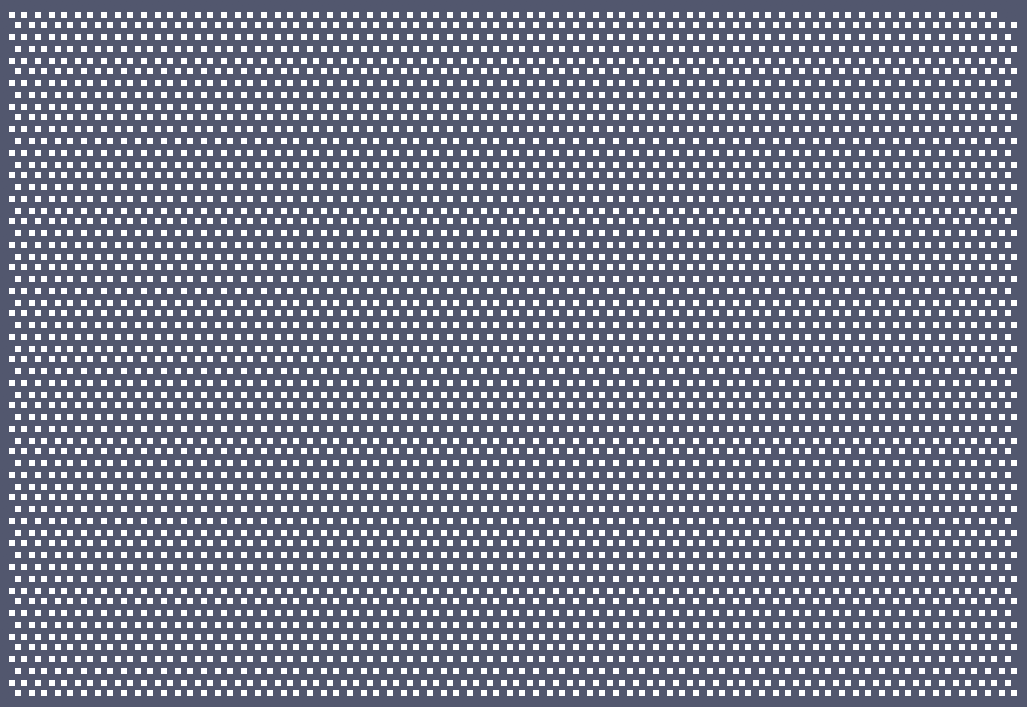
\includegraphics[width=0.7\textwidth]{grid.png}}
\caption{\label{fig:grid}Grid of 4559 points to print.}
\end{figure}


We employ an analytical heat transfer model that simulates a print path and calculates the thermal gradient and solid liquid interface velocity for cells within a geometry. It also outputs a value on a scale between 0 and 1 that indicates the predicted prevalence of equiaxed or columnar microstrucutre – 0 indicating columnar and 1 indicating equiaxed structure. 

For these experiments we aim to manipulate print paths over a fixed set of points to create arbitrary, yet predetermined, microstructure regions. These experiments will show the effectiveness and generalizability of these methods for controlling microstructure. This work explores two distinct methods that can be used independently or in conjunction to manipulate the microstructure. Each method controls a unique component of the print path – spot order and spot time – in order to yield the desired microstructure. For both methods a semi-analytical, finite element model was used to evaluate solutions.

Each experiment had the same initial set of candidate points that filled a 15x10 mm rectangle. The points were laid out on a hexagonal grid with 200 micron spacing between each point. Each solution also began with a spot order that was a random ordering of these 4,559 points. 


\subsection{Control through spot order}
\label{subsec:spotorder}

To optimize the spot order we employed a method called genetic algorithm. The general algorithm is enumerated in algorithm \ref{algo:genetic}. This version of the algorithm has three distinct groups of specimen that are treated differently. Of the entire population \textit{p}, the least fit half are eliminated and not allowed to produce new solutions; the most fit half are allowed to continue. Additionally, this implementation has \textit{q} specimen, the elites, that are the most fit individuals. They remain unchanged through the crossover and mutation phases to ensure that the overall best solutions do not get worse over time. For this implementation to work \textit{q} must be less than \textit{p}/2.


\begin{algorithm}
\caption{Genetic Algorithm}
\label{algo:genetic}
\begin{algorithmic}[1]
\State Generate population of size \textit{p}
\For{\textit{n} generations}
  \State Evaluate fitness for each individual
  \State Determine \textit{q} most fit individuals
  \State Eliminate \textit{p}/2 least fit individuals
  \State Duplicate remaining individuals and randomly pair
  \State Perform pairwise crossover for individuals not in \textit{q}
  \State Perform mutation for each individual not in \textit{q}
\EndFor
\State Perform final fitness evaluation
\State Return most fit individual
\end{algorithmic}
\end{algorithm}


The success of the genetic algorithm can hinge on the ability of the fitness function to mathematically capture what is a good solution. The fitness function must not just evaluate the performance of the solution but also help push the search to regions where solutions are more likely to be found. For this problem we chose to use a two-part fitness function to lead us to these ends. 

\begin{equation}
\label{eq:fitness}
F_{Tot} = \sum_{P} F_{S}(p) + F_{H}(p, p_{prev})
\end{equation}

\begin{equation}
\label{eq:micro}
F_{S}(p) = \begin{cases} 
            -M(p) & \text{if $p \in columnar$} \\
            M(p) - 1 & \text{if $p \in equiaxed$}
            \end{cases}
\end{equation}

\begin{equation}
\label{eq:heuristic}
F_{H}(p, p_{prev}) = \begin{cases} 
                        -\frac{1}{1 + DIST(p, p_{prev})}  & \text{if $p \in columnar$} \\
                        \frac{1}{1 + DIST(p, p_{prev})} - 1 & \text{if $p \in equiaxed$}
                        \end{cases}
\end{equation}

These equations serve to penalize a solution if it has poor simulated results or if it violates a known heuristic (which could subsequently lead to poor offspring in future generations). We chose to weight the two component fitness function equally when evaluating the total fitness of a possible solution. Equation (\ref{eq:fitness}) represents the total fitness. It is the summation of two scores for every point in the print path. 

Equation (\ref{eq:micro}) scores the correctness of the simulated microstructure for a point. The function, $M$, represents the predicted microstructure for that point from the model, and the appropriate equation is chosen depending on the intended microstructure for the point. So, if the microstrucutre is approximately correct then the output of this equation will be negative but close to 0; however, if the predicted microstructure is not similar to the intent then the output will be negative but close to -1.

Finally, equation (\ref{eq:heuristic}) represents the heuristic. It serves to push the solutions to more successful regions of the search space. The basic rationale behind the heuristic is that equiaxed microstrucutre is more like to be achieved when points that are physically close together are also melted close together in time. This allows for larger melt pools and lower thermal gradients. Conversely, columnar microstructure is likely to be produced when points that are physically close together are printed far apart temporally. This yields smaller melt pools and higher thermal gradients (specifically in the Z direction). The function, then, penalizes solutions that violate these principles. This function will output a negative number that is close to 0 if the point follows the rule and close to -1 if it violates it. This ensures, especially at the beginning, that the species that are evolved come from an increasingly suitable set of possible solutions. Overall, the genetic algorithm seeks to generate a solution that maximizes the fitness function.


\subsection{Control through spot time}
\label{subsec:spottime}

To optimize spot time we used a method that we are dubbing “gradient descent” because it follows the basic rationale of its namesake. Our implementation of gradient descent is enumerated in algorithm \ref{algo:graddesc}. 

\begin{algorithm}
\caption{"Gradient Descent"}
\label{algo:graddesc}
\begin{algorithmic}[1]
\State Initialize the base global spot time and the multiplier for every point
\While{changing}
  \State Simulate path
  \For{each point}
    \State Evaluate error from desired microstructure
    \State Increment/decrement multiplier to move toward desired microstructure
  \EndFor
\EndWhile
\State Perform final fitness evaluation and take top result
\end{algorithmic}
\end{algorithm}


Additionally, we perform one iteration of each experiment that utilizes the two methods in conjunction. First, we take the results from the spot order optimization and perform the gradient descent on the solution. We do not perform the inverse experiment because the spot time optimizations, intuitively, are dependent on the spot order, so optimizing spot time first would yield poor results. 

\begin{figure}
\centering
\frame{
\includegraphics[width=0.3\textwidth]{50-50_intent.png}}
\caption{\label{fig:intent50}Binary image for simple microstructure region intent. Black represents columnar, and white represents equiaxed.}
\end{figure}

\begin{figure}
\centering
\frame{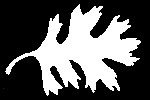
\includegraphics[width=0.3\textwidth]{leaf_intent.png}}
\caption{\label{fig:intentleaf}Binary image for complex microstructure region intent.}
\end{figure}



\section{Experiments}
\label{sec:experiments}

\subsection{Experiment – 50-50}
\label{subsec:exp50-50}

A 50-50 pattern was chosen to simply test the ability of the methods to utilize modeled data and manipulate spot path parameters in order to optimize microstructure – a proof of concept. This geometry is simple, and we have been able to successfully produce it using heuristics and a deterministic algorithm. Therefore, we would be able to compare the results of this method with the previous results. 


\subsection{Experiment – oak leaf}
\label{subsec:expleaf}

The oak leaf pattern was chosen to test the flexibility and generalizability of the methods to regions of arbitrary and complex shape. 


\section{Results}
\label{sec:results}

The following results show the genesis of each method from the initial solution to the final solution. 


\subsection{Experiment – 50-50}
\label{subsec:result50-50}

\begin{table}
\centering
\begin{tabular}{c|c}
\textbf{Method Description} & \textbf{Average Absolute Pixel Error} \\\hline
Spot Order & 0.440\% \\
Spot Time & 0.271\% \\
Spot Order + Spot Time & 0.269\%
\end{tabular}
\caption{\label{tab:result50}An example table.}
\end{table}

\subsection{Experiment – oak leaf}
\label{subsec:resultleaf}

\begin{table}
\centering
\begin{tabular}{c|c}
\textbf{Method Description} & \textbf{Average Absolute Pixel Error} \\\hline
Spot Order & 0.422\% \\
Spot Time & 0.361\% \\
Spot Order + Spot Time & 0.332\%
\end{tabular}
\caption{\label{tab:resultleaf}An example table.}
\end{table}


\begin{figure}
\centering
\frame{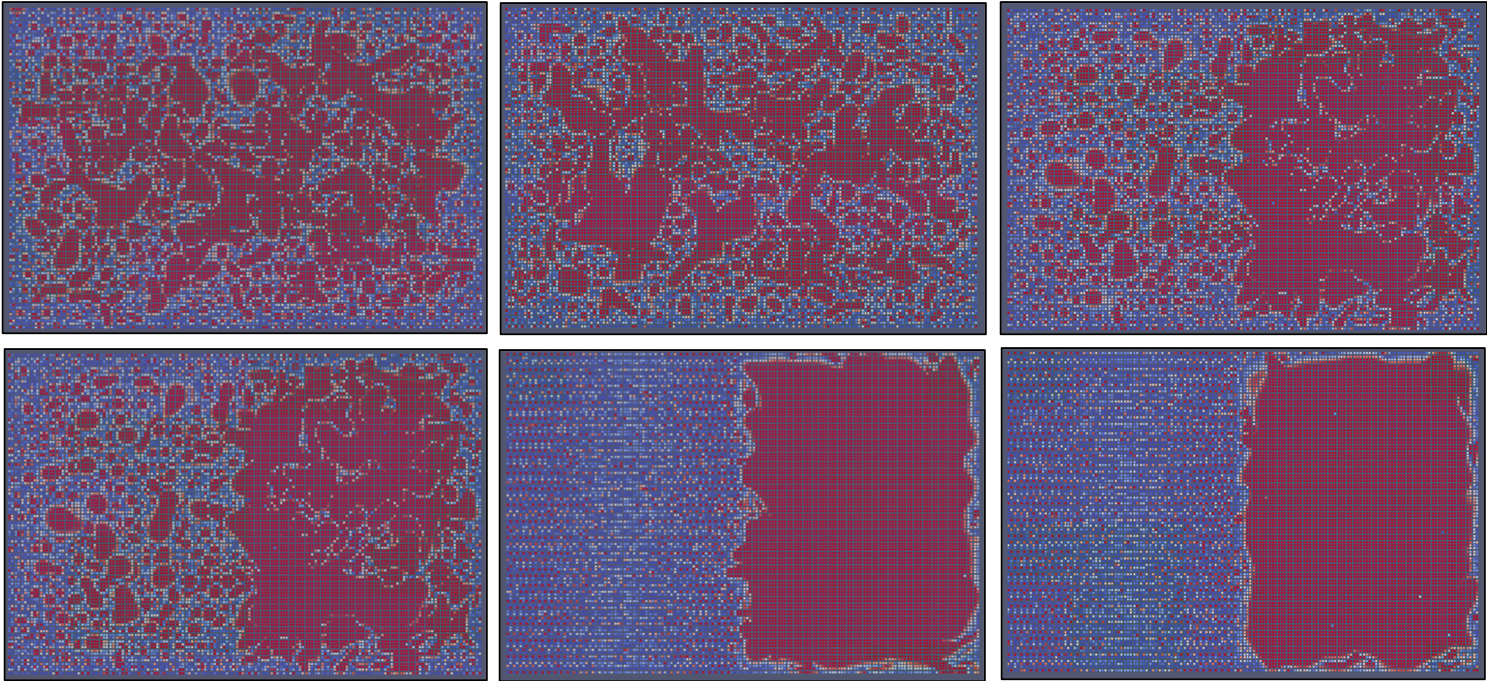
\includegraphics[width=0.7\textwidth]{50-50_results.png}}
\caption{\label{fig:result50}Microstructure before (first row) and after (second row) for spot order (left), spot time (middle), and dual (right) for the simple region.}
\end{figure}

\begin{figure}
\centering
\frame{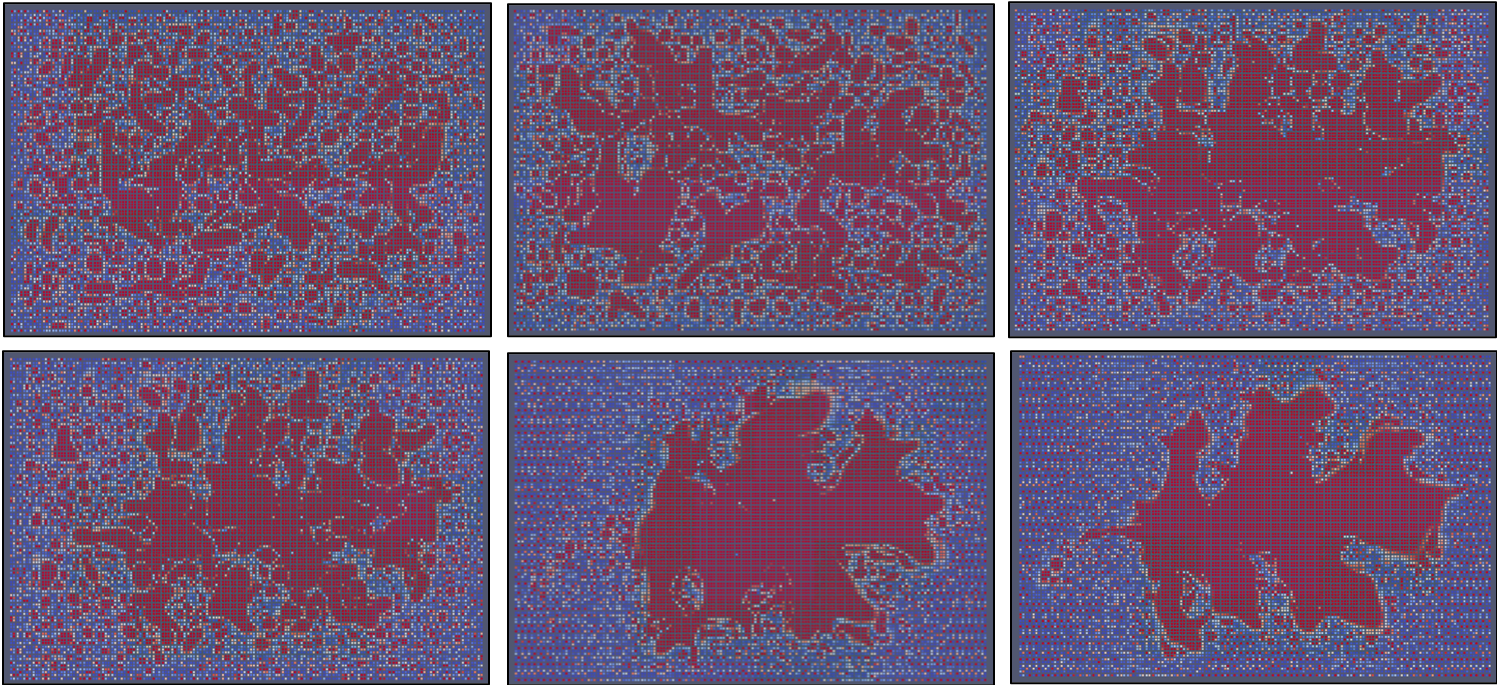
\includegraphics[width=0.7\textwidth]{leaf_results.png}}
\caption{\label{fig:resultleaf}Microstructure before and after for the complex region.}
\end{figure}


\section{Discussion}
\label{sec:discussion}

The genetic algorithm route is absolutely necessary to find a good spot order solution in a reasonable amount of time. Of note is that fact that we only had to simulate approximately 30,000 solutions before landing on the spot order results shown above. For reference, this is approximately 10,000 fewer solutions to test than if one were to try to brute-force enumerate all of the possible permutations of a path consisting of only eight points. So, one can clearly see that reasonable results are found after only searching a minute fraction of the total possible point order space. 


\section{Future Work}
\label{sec:futurework}

-	Analyze the best spot order that we achieved for
o	general


\section{Conclusion}
\label{sec:conclusion}

*columnar/equiaxed in different locations
Geometry independent methods


\bibliographystyle{plain} % We choose the "plain" reference style
\bibliography{references} % Entries are in the "references.bib" file

% \section{DELETE}
% \subsection{How to Make Lists}

% You can make lists with automatic numbering \dots

% \begin{enumerate}
% \item Like this,
% \item and like this.
% \end{enumerate}
% \dots or bullet points \dots
% \begin{itemize}
% \item Like this,
% \item and like this.
% \end{itemize}
% \dots or with words and descriptions \dots
% \begin{description}
% \item[Word] Definition
% \item[Concept] Explanation
% \item[Idea] Text
% \end{description}

% We hope you find write\LaTeX\ useful, and please let us know if you have any feedback using the help menu above.

\end{document}

- include simulation parameters and rationale
- give the necessary information for others to replicate the results (goal of methodology/experiments section)

Strategy for Texture Management in Metals Additive Manufacturing
- point melt good because it is outside of the black box
- point melt parameters can be manipulated to control microstructure (transition from columnar anisotropic to equiaxed isotropic)
- Energy density is the key thing that is "controlled" during dehoff fill point melt
- come up with custom point melt strategies that control the energy density in different regions of a part
- some control has been shown with DOE experiment
- now offering a method of control with point melt
- point melt parameters are beam current, spot time, skip (order), and point spacing
    - we try changing only spot order and spot time to control energy density and subsequent microstrucutre (texture)?
    - so we (may be able to) posit that with "good" beam current and point spacing for a geometry, a combination (or path) comprised of point order and spot time may be found to yield a desired microstructure.
    
Strategy for Texture Management in Metals Additive Manufacturing
- This model can be used to evaluate in fill patterns to see how they interact/affect microstructure
- !! the paper does NOT enumerate how the microstructure is predicted within the model !!
    - we will need to include the equation/reference that tells how the thermal gradient and interface velocity can predict the microstructure that develops
- Assumptions of the model may not extend to complex geometries (=> but should be valid for this work b/c rectangle)
- "This paper proposes a pragmatic alternative based on a semi-analytical approach to predicting the transient heat conduction during powder bed metal additive manufacturing processes."

RAMBLINGS
Additive manufacturing offers the most flexibility of any manufacturing process. It enables the fabrication of geometries that are not possible with conventional methods of manufacturing. Further more, the process allows for the possibility of controlling the formation of microstrucutre for a component during fabrication. In fact, [blank] has also shown the ability ot utilize custom infill pattern for metal additive manufacturing. specifically, they use a spot fill patter that does not rely on the "black box" of software imposed by additive manufacturing machine manufacturers. They deomnstrated how using sucha a technique can allow for the production of either columnar grains with anisotropic tendencies or equiaced grains with isotropic tendencies. However, their approach has limited flexibility because the algorithm of their infill pattern necessitates that the geometry is square or a similarly simple geometry. Additionally, their approach only allows for homogeneous microstrucutre within a layer of a part. [blank] has shown that through metal additive processes that the very microstructure of a part can be controlled and different regions of a layer can have certain mechanical properties imposed upon them. However, the technique employed there is dependant on the proprietary algorithms of ARCAM (wat is arcam? need to introduce some of the concepts better. This paper introduces a method of microstructure control that is more general than any of these previous efforts. It utilizes the spot infil method (as opposed to proprietary rasterization techniques).